In this exercise we write discrete event simulation program for a blocking system,with n service units and no waiting room.\\
First, the arrival process is modelled as a Poisson process and the service time distribution is modeled as exponential for $n = 10$(number of service units), mean service time = 8 time units, mean time between customers = 1 time unit and 10.000 customers, then record the fraction of blocked customers, and a confidence
interval for this fraction.\\
In the second part of this exercise, we substitute the arrival process with a renewal process with\\
1:Erlang distributed inter arrival times mean of 1\\
2:hyper exponential inter arrival times with $p_1 = 0.8$, $\lambda_1 = 0.8333$, $p_2 = 0.2$, $\lambda_2 = 5.0$.\\
Finally experiment with different service time distributions.
Suggestions are constant service time and Pareto distributed service times with k = 1.05 and k = 2.05.\\
All this results is presented in Table 4.\\

\begin{center}
    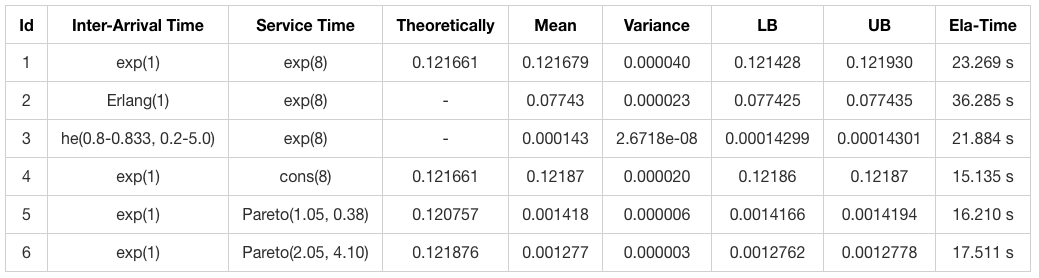
\includegraphics[scale=0.5]{Figures/figure4_1.png}\\
    \figuretitle{Table 4 :Discrete Event Simulation of Blocking System .}
\end{center}\\
\\
\begin{center}
    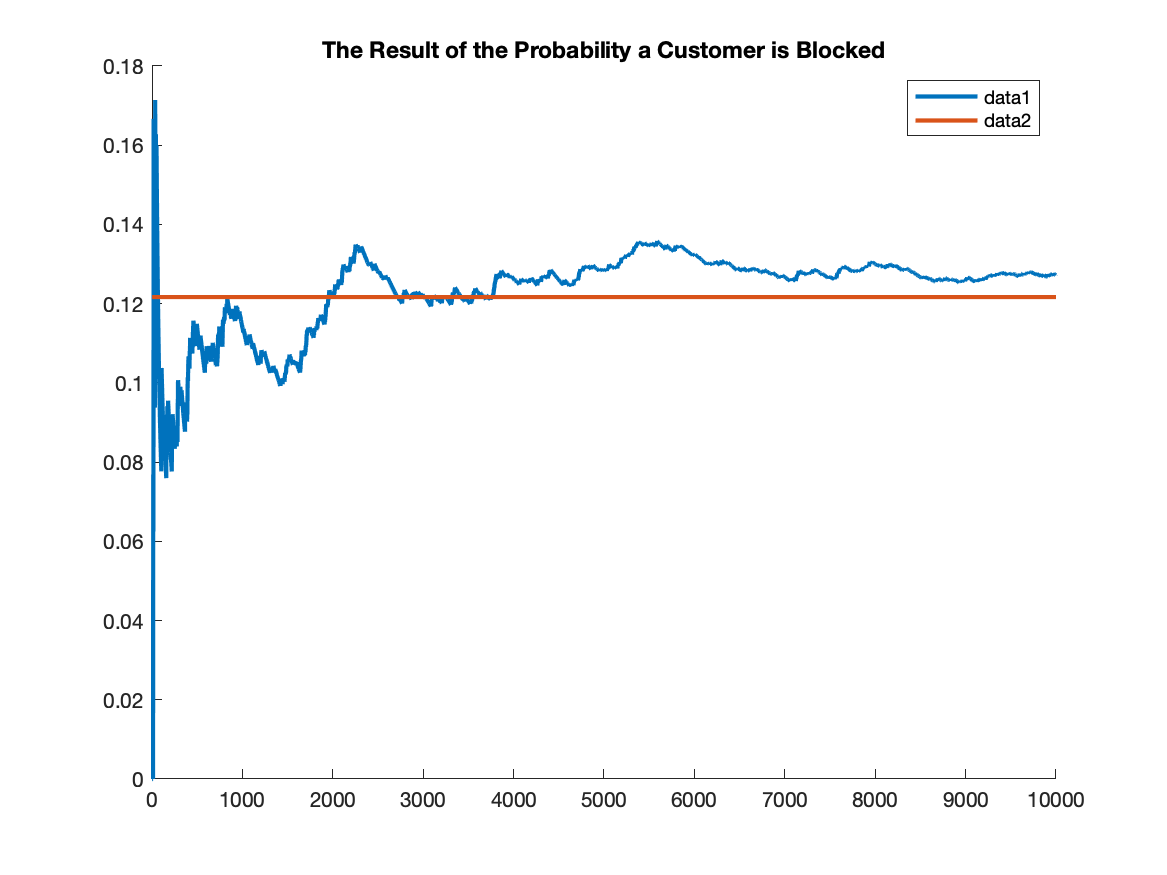
\includegraphics[scale=0.4]{Figures/figure4_2.png}\\
    \figuretitle{Figure 12: The result of the probability a customer is blocked.}
\end{center}\\
\\


%\begin{table}[h!]
%\centering
%\caption{Discrete Event Simulation of Blocking System .}
%\label{summstats}
%\begin{tabular}{|l|c|c|c|c|c|c|c|}
%\hline
%\textbf{Series}  & \multicolumn{1}{l|}{\textbf{Inter-Arrival Time}} & \multicolumn{1}{l|}{\textbf{Service Time}}& %\multicolumn{1}{l|}{\textbf{Mean}}& \multicolumn{1}{l|}{\textbf{Variance}}& \multicolumn{1}{l|}{\textbf{Lower Bound}}& %\multicolumn{1}{l|}{\textbf{Upper Bound}} & \multicolumn{1}{l|}{\textbf{elapsed time}}\\ \hline

   % Analysis      & \exp{1}& \exp{8}   & 0.121661  & - & -         & -        & -       \\ \hline
   % 1 &  exp(1)   & exp(8) & 0.121679  & 0.000040  & 0.121428  & 0.121930 & 23.269 s \\  \hline
   % 2 & Erlang(1) & exp(8) & 1.000343  & 0.000020  & 1.000164  & 1.000523 & 39.241 s \\  \hline
    %3 & he(0.8-0.833, 0.2-5.0) & exp(8) & 4.163967  & 0.002352  & 4.162038  & 4.165897 & 24.459 s \\  \hline
    %4 & exp(1)    & cons(8) & 0.999592  & 0.000081  & 0.999234  & 0.999951 & 16.072 s \\  \hline
    %5 & exp(1)    & Pareto(1.05, 0.38) & 1.001194  & 0.000071  & 1.000859  & 1.001529 & 17.601 s \\  \hline
    %6 & exp(1)    & Pareto(2.05, 4.10) & 0.998682  & 0.000109  & 0.998267  & 0.999098 & 19.684 s \\  \hline
%\end{tabular}
%\end{table}\\
\\
